% Options for packages loaded elsewhere
\PassOptionsToPackage{unicode}{hyperref}
\PassOptionsToPackage{hyphens}{url}
\documentclass[
]{ltjsarticle}
\usepackage{xcolor}
\usepackage{amsmath,amssymb}
\setcounter{secnumdepth}{-\maxdimen} % remove section numbering
\usepackage{iftex}
\ifPDFTeX
  \usepackage[T1]{fontenc}
  \usepackage[utf8]{inputenc}
  \usepackage{textcomp} % provide euro and other symbols
\else % if luatex or xetex
  \usepackage{unicode-math} % this also loads fontspec
  \defaultfontfeatures{Scale=MatchLowercase}
  \defaultfontfeatures[\rmfamily]{Ligatures=TeX,Scale=1}
\fi
\usepackage{lmodern}
\ifPDFTeX\else
  % xetex/luatex font selection
\fi
% Use upquote if available, for straight quotes in verbatim environments
\IfFileExists{upquote.sty}{\usepackage{upquote}}{}
\IfFileExists{microtype.sty}{% use microtype if available
  \usepackage[]{microtype}
  \UseMicrotypeSet[protrusion]{basicmath} % disable protrusion for tt fonts
}{}
\makeatletter
\@ifundefined{KOMAClassName}{% if non-KOMA class
  \IfFileExists{parskip.sty}{%
    \usepackage{parskip}
  }{% else
    \setlength{\parindent}{0pt}
    \setlength{\parskip}{6pt plus 2pt minus 1pt}}
}{% if KOMA class
  \KOMAoptions{parskip=half}}
\makeatother
\usepackage{longtable,booktabs,array}
\newcounter{none} % for unnumbered tables
\usepackage{calc} % for calculating minipage widths
% Correct order of tables after \paragraph or \subparagraph
\usepackage{etoolbox}
\makeatletter
\patchcmd\longtable{\par}{\if@noskipsec\mbox{}\fi\par}{}{}
\makeatother
% Allow footnotes in longtable head/foot
\IfFileExists{footnotehyper.sty}{\usepackage{footnotehyper}}{\usepackage{footnote}}
\makesavenoteenv{longtable}
\usepackage{graphicx}
\makeatletter
\newsavebox\pandoc@box
\newcommand*\pandocbounded[1]{% scales image to fit in text height/width
  \sbox\pandoc@box{#1}%
  \Gscale@div\@tempa{\textheight}{\dimexpr\ht\pandoc@box+\dp\pandoc@box\relax}%
  \Gscale@div\@tempb{\linewidth}{\wd\pandoc@box}%
  \ifdim\@tempb\p@<\@tempa\p@\let\@tempa\@tempb\fi% select the smaller of both
  \ifdim\@tempa\p@<\p@\scalebox{\@tempa}{\usebox\pandoc@box}%
  \else\usebox{\pandoc@box}%
  \fi%
}
% Set default figure placement to htbp
\def\fps@figure{htbp}
\makeatother
\setlength{\emergencystretch}{3em} % prevent overfull lines
\providecommand{\tightlist}{%
  \setlength{\itemsep}{0pt}\setlength{\parskip}{0pt}}
\usepackage{bookmark}
\IfFileExists{xurl.sty}{\usepackage{xurl}}{} % add URL line breaks if available
\urlstyle{same}
\hypersetup{
  hidelinks,
  pdfcreator={LaTeX via pandoc}}

\author{}
\date{}

\begin{document}

\section{論文12：双子最小空間モデル}\label{ux8ad6ux658712ux53ccux5b50ux6700ux5c0fux7a7aux9593ux30e2ux30c7ux30eb}

\subsection{安定種の外部像・測定の厳密形・もつれのレイヤ解消・頂点の不足と隠れ二軸
---
量子的挙動の界面創発}\label{ux5b89ux5b9aux7a2eux306eux5916ux90e8ux50cfux6e2cux5b9aux306eux53b3ux5bc6ux5f62ux3082ux3064ux308cux306eux30ecux30a4ux30e4ux89e3ux6d88ux9802ux70b9ux306eux4e0dux8db3ux3068ux96a0ux308cux4e8cux8ef8-ux91cfux5b50ux7684ux6319ux52d5ux306eux754cux9762ux5275ux767a}

著者: 木原 範昭 (Noriaki Kihara) 所属: WF System Co., Ltd. ORCID:
0009-0004-6753-4020 版: v0.2 日付: 2026 年 6 月 DOI（本版）: 10.5281/zenodo.20640469
Concept DOI: 10.5281/zenodo.20640468 ライセンス: CC BY 4.0

\begin{center}\rule{0.5\linewidth}{0.5pt}\end{center}

\subsection{要旨}\label{ux8981ux65e8}

本稿はシリーズの最終篇として、二つの複合体が共存する最小の系 ---
\textbf{双子最小空間モデル} ---
を構成し、量子力学的に見える挙動のどこまでが、振幅も連続時間も仮定しない離散関係模型の\textbf{階層界面の読み}として導出されるかを検証する。

\textbf{安定種の外部像}：複合体を外から観測する取っ手（毛）は三つの帳簿に分かれる。面の基本波
\(\nu_0=1/(2\sqrt s)\)（自容器スペクトルの支配線）、親記録の線
\(\nu_{\mathrm{obs}}=|k|\)、エネルギー様ノルム \(R'=\sqrt s\)
である。厳密恒等式 \(\nu_0 R'=1/2\)（零点）が前二者を結び、\(R'\)
は線としては現れず\textbf{奇数コムの間隔 \(1/R'\)
として}外部から読める（記録定理の粒子レベルの実現）。外部像は、間隔
\(1/R'\) の奇数コムを内蔵し広がり \(2R'\)
に局在する\textbf{最小不確定性の準矩形波束}である（半幅×基本波＝\(1/2\)）。

\textbf{双子系の構成}：初期値 \(\Omega_0^2=2\nu_1^2=18\)
は偶数ラベルであり、分類定理（論文5）により単一状態として存在できない
---
\textbf{対として生まれることがパリティで強制される}（最初のイベントに動力学は不要）。双子（各
\(s=9\)）の許される格子分離は \(|\Delta|^2\in\{2,\ldots,20\}\)
に量子化され、\(|\Delta|^2\equiv1\pmod4\)
は全面禁止される。18の関係クラスは縞データのみで完全分離する ---
\textbf{空間の目盛りは等周波数殻の弦集合として生まれる}。

\textbf{測定の厳密形}：測定の二条件（系への影響、変化の検知）を検査すると、変化の検知は前状態の知識を要して無限後退するが、本モデルでは前状態の記録が検閲により不在であり、\(\lambda\)
帳簿は追記専用（単調増加定理、論文6）であるため、後退は構造的に切断される。\textbf{測定＝記録の追記（無→有）}であり、「収縮」は記録の出現、その不可逆性は時間の矢と同一の1ビットに還元される。双子の最初の崩壊を明示計算すると、参照波（\(s=1\)）の出現により記録の情報クラスが干渉計的→ホログラフィック型に昇格する
---
\textbf{測定装置はイベント自身が生む}。あわせて、終状態統計が測度の選択（一括の配置等重率
60/61 対 逐次の条件付き数え上げ
396/403）に依存すること（\textbf{測度分岐}、差 \(+0.00098\)
厳密）を示す。

\textbf{もつれのレイヤ解消}：単一断片の自己スペクトルは全成分偶数ベクトルに乗るため、論理波（奇数）セクターでは恒等的に不可視である
---
\textbf{読めるのは計数と関係のみ}（関係限定読み出し定理）。一方の崩壊は他方の分岐統計を瞬時に書き換える（全変動
0.774）が、このシフトは\textbf{双子の分離に一切依存せず}、影響は子レイヤの空間を伝播していない
---
瞬時性は速度ではなくレベルの不一致である。順序・帰属は最終記録に存在しないため操作的無信号性が従う。もつれた対は偶数ラベルゆえ上のレイヤで単一粒子になれない（パリティ保護）。同じ写像は単一波束の二経路干渉にも適用される。

\textbf{頂点の不足と隠れ二軸}：イベント前後の記録連続則（親の同一性の線が娘系の交差スペクトルに存続すること）を全数検査すると、存続条件として\textbf{位置ベクトルの保存則
\(v_5\pm v_3=\pm v_9\)（運動量類似）が導出され}、\((2,1,0,0)\)
軌道の親では成立するが \((1,1,1,1)\)
軌道の親では\textbf{ちょうど1単位}（1軸／1量子）不足して成立しない。さらに励起次数
\(\varepsilon=(-1)^{\Sigma|k|}\)
の簿記には、これと\textbf{独立な}第二の1ビット不足が存在する（s=7, 9
の特定軌道）。可視4軸の帳簿は二つの不可視方向 --- 曲率側 R
と裸パリティ側 Q ---
を要求しており、不可視方向に沿った中間変位は記録されないため許容される（\textbf{仮想変位の認可原理}）。この認可は、可視帳簿で禁止されている2体分裂を仮想的に解禁し、\textbf{全ての崩壊を3次頂点の列に分解する}（同一終状態への複数経路）。

最後に、得られた構造の標準理論との対応を\textbf{移送原理}（前提の対応物が検証済みなら定理は移送される）として整理し、本モデルが標準理論の側では公準にとどまる問い（測定問題・切断の位置・時間問題・次元・測度）に与える解答候補を、反証可能性（重力媒介もつれ実験等）と併せて明示する。

\begin{center}\rule{0.5\linewidth}{0.5pt}\end{center}

\subsection{キーワード}\label{ux30adux30fcux30efux30fcux30c9}

複合粒子、波束、関係的観測量、測定問題、無信号性、もつれ、Bell
不等式、仮想状態、隠れ次元、Kaluza--Klein、構造対応

\begin{center}\rule{0.5\linewidth}{0.5pt}\end{center}

\subsection{1. はじめに}\label{ux306fux3058ux3081ux306b}

逆数双対モデル（論文4 {[}1{]}
までで導入）に対するシリーズの到達点（論文5--11
{[}2{]}）は、離散・無時間・振幅なしの関係模型に、離散スペクトル・不確定性の床・排他統計・ゲージ構造・次元選択が定理として備わることであった。本稿の問いは最終段である：

\begin{quote}
量子力学に固有とされる挙動 ---
波束、測定の不可逆性、もつれの非局所相関、仮想状態 ---
のうち、どこまでがこの模型の\textbf{階層界面の読み}として導出され、どこからが本質的に新しい入力を要するか。
\end{quote}

方法論上の鍵は二つある。第一に、\textbf{最小の二体系}を使うこと：等しい代表周波数を持つ双子は、未決の時計問題を設定から消し、純粋な関係観測量だけを残す。第二に、\textbf{記録}を一貫した審級とすること：観測量とは記録可能量である（論文6）。

関連する文脈：測定問題と測定の連鎖（von Neumann
{[}5{]}）、デコヒーレンスによる古典性の創発（Zurek {[}6{]}）、Bell
の定理と CHSH 不等式 {[}7,8{]}、重力起因の状態収縮仮説（Penrose
{[}9{]}）と重力媒介もつれの実験提案（Bose ら {[}10{]}、Marletto \&
Vedral {[}11{]}）、経路積分における仮想中間状態（Feynman
{[}12{]}）、余剰次元からの電荷（Kaluza {[}13{]}、Klein
{[}14{]}）、情報を基礎に置く視点（Wheeler
{[}4{]}）。本稿はこれらの理論の拡張ではなく、有限模型の全数計算がこれらの\textbf{構造}をどこまで再現するかの検査である。

\begin{center}\rule{0.5\linewidth}{0.5pt}\end{center}

\subsection{2.
安定種の外部像：三つの帳簿と波束}\label{ux5b89ux5b9aux7a2eux306eux5916ux90e8ux50cfux4e09ux3064ux306eux5e33ux7c3fux3068ux6ce2ux675f}

\subsubsection{2.1
三つの代表周波数と恒等式}\label{ux4e09ux3064ux306eux4ee3ux8868ux5468ux6ce2ux6570ux3068ux6052ux7b49ux5f0f}

安定種
\(s=1,3,5\)（論文7）を外部から観測する取っ手は三つある（自容器スペクトルの厳密計算による）：

{\def\LTcaptype{none} % do not increment counter
\begin{longtable}[]{@{}
  >{\raggedright\arraybackslash}p{(\linewidth - 8\tabcolsep) * \real{0.1667}}
  >{\raggedleft\arraybackslash}p{(\linewidth - 8\tabcolsep) * \real{0.2222}}
  >{\raggedleft\arraybackslash}p{(\linewidth - 8\tabcolsep) * \real{0.2222}}
  >{\raggedleft\arraybackslash}p{(\linewidth - 8\tabcolsep) * \real{0.2222}}
  >{\raggedright\arraybackslash}p{(\linewidth - 8\tabcolsep) * \real{0.1667}}@{}}
\toprule\noalign{}
\begin{minipage}[b]{\linewidth}\raggedright
量
\end{minipage} & \begin{minipage}[b]{\linewidth}\raggedleft
\(s=1\)
\end{minipage} & \begin{minipage}[b]{\linewidth}\raggedleft
\(s=3\)
\end{minipage} & \begin{minipage}[b]{\linewidth}\raggedleft
\(s=5\)
\end{minipage} & \begin{minipage}[b]{\linewidth}\raggedright
地位
\end{minipage} \\
\midrule\noalign{}
\endhead
\bottomrule\noalign{}
\endlastfoot
面の基本波 \(\nu_0=1/(2\sqrt s)\) & 0.5000 & 0.2887 & 0.2236 &
自容器スペクトルの支配線 \\
親記録の線 \(\nu_{\mathrm{obs}}=\lvert k\rvert\) & 0（DC） & 1 &
\(\sqrt2\) & 親の単位記録に現れる線 \\
ノルム \(R'=\sqrt s\) & 1 & 1.732 & 2.236 &
保存帳簿。\textbf{線としては現れない} \\
\end{longtable}
}

厳密恒等式
\(\nu_0R'=1/2\)（零点）が面帳簿とノルム帳簿を結ぶ。\(\nu=\sqrt s\)
は面の梯子の偶数段に当たり奇数スペクトルに存在しない ---
エネルギー様の量は線の位置ではなく、\textbf{奇数コムの間隔
\(1/R'\)}（すなわち λ
側の延長量）として読まれる。これは記録定理（論文6：\(\nu\) は
\(\lambda\)
配置としてのみ記録される）の粒子レベルでの実現である。なお純奇数コムは
\(s=1\) のみであり、複合体はコムのパリティ汚染率（\(s=3\) で
49\%、\(s=5\) で 21\%）として\textbf{複合性を外部に署名する}。

\subsubsection{2.2
波束としての外部像}\label{ux6ce2ux675fux3068ux3057ux3066ux306eux5916ux90e8ux50cf}

外部像は、(i) 有限の広がり \(2R'\) に局在し、(ii)
通約的な奇数コムにより周期 \(2R'\) ごとに厳密に自己復元し、(iii)
半幅×基本波＝\(1/2\)
の\textbf{最小不確定性}に飽和する、準矩形の孤立波束である。形状を保つ機構は非線形性ではなく検閲（論文9）である。エネルギーラベルは零点ドレッシング公式
\(s=\nu_{\mathrm{obs}}^2+\|k\|_1+1\) により親記録の線から推定される。

\begin{figure}
\centering
\pandocbounded{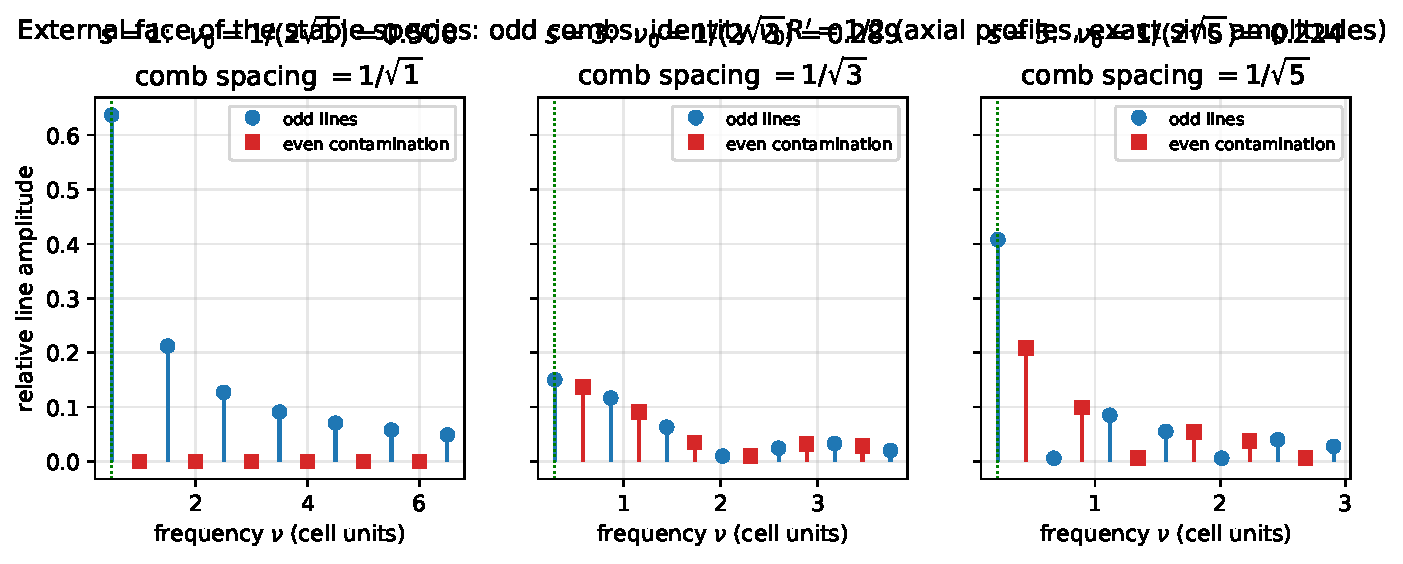
\includegraphics[keepaspectratio,alt={Figure 1. External face of the stable species: odd combs}]{figure_paper12_1_species_combs.pdf}}
\caption{Figure 1. External face of the stable species: odd combs}
\end{figure}

\textbf{図1. 安定種の外部像（軸断面の厳密 sinc 振幅）：奇数コムの間隔
\(1/\sqrt s\) が \(R'\)
を、偶数線の汚染率が複合性を外部に伝える。緑点線＝基本波
\(\nu_0=1/(2\sqrt s)\)。}

\begin{center}\rule{0.5\linewidth}{0.5pt}\end{center}

\subsection{3.
双子最小空間モデル}\label{ux53ccux5b50ux6700ux5c0fux7a7aux9593ux30e2ux30c7ux30eb}

\subsubsection{3.1
パリティによる対生成の強制}\label{ux30d1ux30eaux30c6ux30a3ux306bux3088ux308bux5bfeux751fux6210ux306eux5f37ux5236}

初期値として単一の振動数 \(\Omega_0\) のみを持つ系を考え、保存則
\(\Omega_0^2=2\nu_1^2=18\) で二つの \(s=9\)
複合体に分かれる状況を設定する。\(S=18\)
は偶数であり、分類定理（論文5）により\textbf{単一状態のスロットを持たない}。したがって
d=4 の格子上では、この系は単一でいる選択肢が運動学的に存在しない ---
「割れる」のではなく\textbf{対として生まれる}。最初のイベントは動力学を要しない。

\begin{figure}
\centering
\pandocbounded{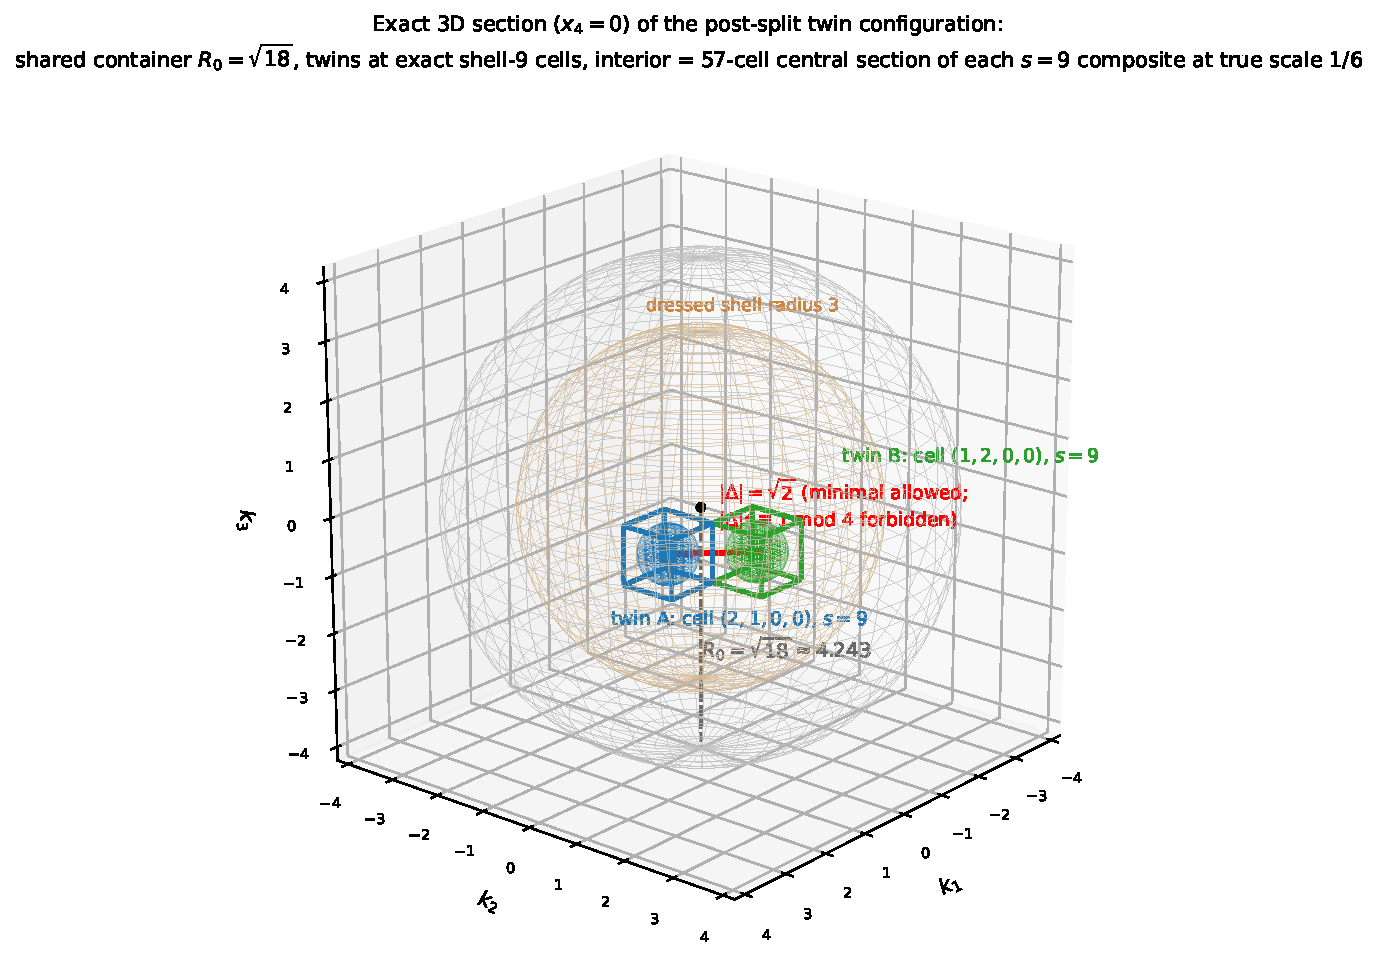
\includegraphics[keepaspectratio,alt={Figure 2. Exact 3D section of the post-split twin configuration at true scale}]{figure_paper12_2_twin_configuration.pdf}}
\caption{Figure 2. Exact 3D section of the post-split twin configuration
at true scale}
\end{figure}

\textbf{図2. 分裂後の双子配置の厳密な3次元断面（\(x_4=0\)）。} 共有容器
\(R_0=\sqrt{18}\approx4.243\)（自己無撞着
\(R_0^2=S=18\)、外側球）の中で、双子は shell-9 セル \((2,1,0,0)\) と
\((1,2,0,0)\) を占有する。分離は最小許容値
\(|\Delta|=\sqrt2\)（\(|\Delta|^2=1\) は mod 4
選択則により禁止）。各双子の単位セル内部には、一階層下の \(s=9\)
複合体（137セル）の中心3次元断面（57立方体）と内部容器（直径1＝内部単位で
\(2R_1=6\)）を縮尺 \(1/6\) で厳密に描いた。内側の球は dressed
殻半径3。位置・間隔・縮尺はすべて厳密計算値であり、論文4 図3
の階層的状態空間の本モデルにおける具体化である。

\subsubsection{3.2 分離スペクトルと mod 4
選択則}\label{ux5206ux96e2ux30b9ux30daux30afux30c8ux30ebux3068-mod-4-ux9078ux629eux5247}

双子は両方とも shell-9（64セル）に乗る。可能な対 \(\binom{64}{2}=2016\)
の全数分類により：

\begin{itemize}
\tightlist
\item
  許される分離
  \(|\Delta|^2\in\{2,3,4,6,7,8,10,11,12,14,15,16,18,20\}\)。
\item
  \textbf{\(|\Delta|^2\equiv1\pmod4\)（隣接 \(1\)
  を含む）は全面禁止}（shell-9
  の2軌道のパリティ構造による：同型対は偶差、異型対は
  \(\equiv3\pmod4\)）。
\item
  \(B_4\)×入替で18の関係クラスに分解され、縞データ
  \((|\Delta|^2,|\Sigma|^2)\) のみで\textbf{完全分離}する（内積
  \(=(|\Sigma|^2-|\Delta|^2)/4\) として角度も縞から直読できる）。
\end{itemize}

\begin{quote}
等しい代表周波数を持つ二実体が取りうる相対位置は、等周波数殻の弦集合として量子化され、禁止帯を持つ。\textbf{この双子系で「距離」として実在する（＝記録に現れる）ものは、この離散カタログがすべてである。}
\end{quote}

\begin{figure}
\centering
\pandocbounded{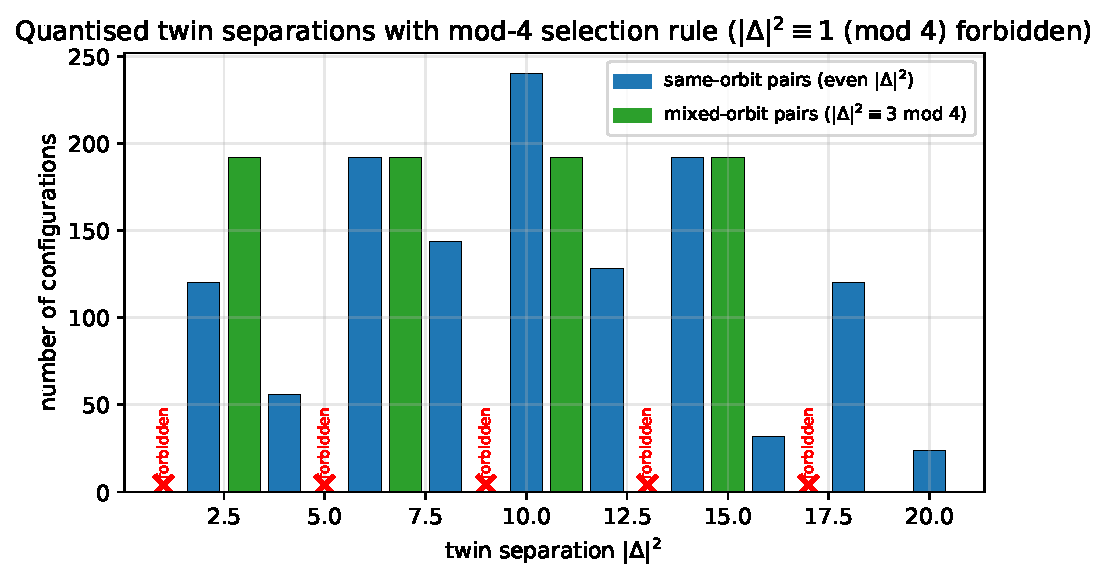
\includegraphics[keepaspectratio,alt={Figure 3. Quantised twin separations with the mod-4 selection rule}]{figure_paper12_3_separation_spectrum.pdf}}
\caption{Figure 3. Quantised twin separations with the mod-4 selection
rule}
\end{figure}

\textbf{図3.
双子分離スペクトル（2016配置の全数）：\(|\Delta|^2\equiv1\ (\mathrm{mod}\ 4)\)
は全面禁止。同型対（偶 \(|\Delta|^2\)）と混合軌道対（\(\equiv3\) mod
4）。}

なお双子系には
\(s=1\)（DC参照）が含まれないため、記録は干渉計的型（関係のみ）であり、DC=2
が「二つあること」を直読する --- 参照なしの最小の二経路干渉計である。

\begin{center}\rule{0.5\linewidth}{0.5pt}\end{center}

\subsection{4.
時計の帳簿とシュレーディンガー方程式の地位}\label{ux6642ux8a08ux306eux5e33ux7c3fux3068ux30b7ux30e5ux30ecux30fcux30c7ux30a3ux30f3ux30acux30fcux65b9ux7a0bux5f0fux306eux5730ux4f4d}

\subsubsection{4.1
関係時計の比}\label{ux95a2ux4fc2ux6642ux8a08ux306eux6bd4}

このモデルに連続時間はなく、時間はイベント計数である（論文6）。よって「位相発展」は背景時間の関数ではなく、\textbf{部分系の位相が他の部分系（時計）に対して進む比}としてのみ意味を持つ（Page--Wootters
型の関係時間 {[}3{]} の最小実装）。候補時計は三つあり、(i)
ノルム時計（\(\nu=\sqrt s\)：重い方が速い）、(ii)
面時計（\(\nu=1/(2\sqrt s)\)：軽い方が速い）、(iii)
裸線時計（\(\nu=|k|\)：軌道型に依存）である。検査の結果：

\begin{itemize}
\tightlist
\item
  \textbf{面時計は消去される}：カスケード（論文8）を面時計で読むと時間が有限値に飽和し、輻射則整合（\(a\propto t^{1/2}\)）を満たす大域時計はノルム時計のみである。
\item
  \textbf{ノルム/面の選択はゲージである}：両者は
  \(\nu_{\mathrm{norm}}\nu_{\mathrm{face}}=1/2\)
  で零点共役であり、大域反転はすべての比を逆数化するラベル替えにすぎない。非ゲージ的内容は「どちらの側が加法的か」の1ビット
  --- 保存の算術はノルム側を選び、連続極限の位相回転則は
  \(\omega\propto\sqrt s\)（エネルギー様）となる。
\item
  \textbf{裸線時計は実差を予言する}：同エネルギーでも軌道型が違えば
  \(|k|\) が違う（shell-9 で 2 対
  \(\sqrt5\)）ため、\textbf{等エネルギーの双子がビートする}。判別器は
  §3.2 の mod 4 構造そのもの（奇 \(|\Delta|^2\)
  クラス＝混合軌道対のみがドリフトしうる）であり、判別にはイベント間の位相接続則を要する（§7）。
\end{itemize}

\subsubsection{4.2
シュレーディンガー方程式は三条件つき有効補間である}\label{ux30b7ux30e5ux30ecux30fcux30c7ux30a3ux30f3ux30acux30fcux65b9ux7a0bux5f0fux306fux4e09ux6761ux4ef6ux3064ux304dux6709ux52b9ux88dcux9593ux3067ux3042ux308b}

\begin{enumerate}
\def\labelenumi{(\roman{enumi})}
\tightlist
\item
  関係時計の部分系が多状態（\(N\gg1\)）、(ii) 検閲下で単一の代表 \(\nu\)
  が複合体を代表できる、(iii)
  離散の目盛りが相対的に微小（\(\varepsilon\sim1/(2\sqrt s)\)）、の三条件の極限で、イベント計数の位相帳簿は連続時間の波動方程式として補間可能になる。補正は
  \(O(\varepsilon)\)
  で小さいだけでなく\textbf{検閲により記録不能}であり、記録のレベルでは厳密に成立して見える（二重保護）。出るのは波動セクター（1粒子の波動方程式相当）のみであり、配置（履歴）にまたがる線形重ね合わせはこの極限からは出ない。破れの予言：少数状態系どうし、階層をまたぐ過程、禁止帯近傍（論文9）。
\end{enumerate}

\begin{center}\rule{0.5\linewidth}{0.5pt}\end{center}

\subsection{5.
測定の厳密形：無→有}\label{ux6e2cux5b9aux306eux53b3ux5bc6ux5f62ux7121ux6709}

\subsubsection{5.1
二条件と後退の切断}\label{ux4e8cux6761ux4ef6ux3068ux5f8cux9000ux306eux5207ux65ad}

測定には二条件が要る：(1) 系と相互作用すること、(2)
状態が変わったと分かること。条件 (2)
は前状態の知識を要し、それも測定であるから無限後退する ---
唯一可能な検知は\textbf{無が有になること}である。本モデルではこの分析がそのまま定理になる：

\begin{enumerate}
\def\labelenumi{\arabic{enumi}.}
\tightlist
\item
  イベント前の複合体の内部は検閲により雲であり、前状態の記録は\textbf{原理的に不在}（比較すべき台帳がない）。
\item
  \(\lambda\) 帳簿は\textbf{追記専用}である（\(\Sigma\lambda^2\)
  の厳密単調増加、論文6）。帳簿に存在する取引はただ一種類 ---
  追記＝無→有。
\end{enumerate}

\begin{quote}
\textbf{測定の厳密形}: 測定とは \(\lambda\)
帳簿への追記イベントである。「収縮」とは記録の出現であり、その不可逆性は時間の矢と同一の1ビットに還元される（公準が一個減る）。Heisenberg
切断の位置の任意性は、階層管轄の境界（検閲が定義する）に対応する。実測定がすべて出現の計数（クリック・乾板の粒）に終端する事実
{[}5{]} と整合する。
\end{quote}

\subsubsection{5.2
最初の測定の明示計算}\label{ux6700ux521dux306eux6e2cux5b9aux306eux660eux793aux8a08ux7b97}

双子Aの崩壊 \(9\to(5,3,1)\) の前後で：DC（断片数）\(2\to4\)、記録の線
\(2\to9\)
本（出現9・消失2）、\(\Sigma\lambda^2=2/9\to74/45\)（厳密増加）、\(\Sigma\nu^2=18\)（保存）。決定的なのは情報クラスの昇格である：\(s=1\)＝参照波の出現により、記録は干渉計的型から\textbf{ホログラフィック型}（全配置復元可、論文7
§6.5；参照波による再構成は Gabor のホログラフィー {[}15{]}
との構造対応）へ変わる。\textbf{この系の最初の崩壊と最初の測定は同一イベントであり、測定装置（参照波）はイベント自身が生む。}
なお消失した線は「読むものを残さない」 ---
存在する記録は現在読めるが、消失の検知は前の記録を要して後退する。出現だけが非対称に読める理由はここにある。

\begin{figure}
\centering
\pandocbounded{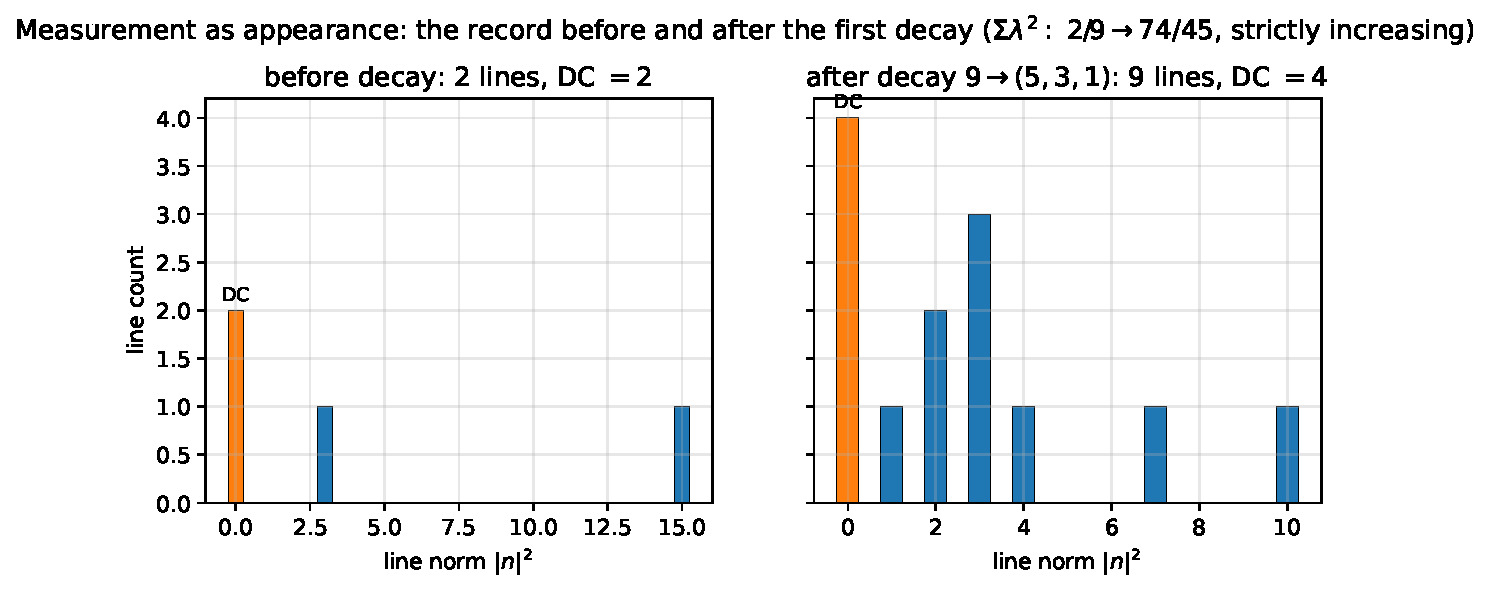
\includegraphics[keepaspectratio,alt={Figure 4. Measurement as appearance: the record before and after the first decay}]{figure_paper12_4_measurement.pdf}}
\caption{Figure 4. Measurement as appearance: the record before and
after the first decay}
\end{figure}

\textbf{図4. 測定＝出現：最初の崩壊 \(9\to(5,3,1)\)
の前後の記録線。DC（断片数）は \(2\to4\)、線は \(2\to9\)
本、\(\Sigma\lambda^2\) は \(2/9\to74/45\) と厳密増加。}

なお本節の代表配置（\(v_3=e_3\)）は等重率下の一例であり、§7.1
の記録連続則を頂点規則として採る場合には認可配置（親 \((2,1,0,0)\)
型では \(v_3=\pm e_1\) 等）で引き直される。DC 増分・\(\Sigma\lambda^2\)
の厳密増加・ホログラフィック昇格という本節の結論は、配置の選択に対して頑健である。

\subsubsection{5.3 測度分岐}\label{ux6e2cux5ea6ux5206ux5c90}

双子の二段崩壊の終状態統計を厳密有理数で比較すると、一括（終配置の等重率）は
\(P=60/61=0.98361\)、逐次（条件付き数え上げ）は
\(396/403=0.98263\)、経路等重は \(0.96000\) ---
\textbf{一致しない}（一括対逐次の差
\(+0.00098\)）。無時間の数え上げ原理は単独では測度を一意に定めず、「イベントの実在構造」（一回か逐次か）が観測可能な差を生む。標準理論はこの問いに導出された答えを持たず（記録された中間なら逐次、なければ経路和、という運用規則の境界＝切断は未導出
{[}5,6{]}）、本モデルでは「記録の有無が合成則を選ぶ」ことが導出可能な見込みの解答候補である（記録が定理水準の概念であるため）。

\begin{center}\rule{0.5\linewidth}{0.5pt}\end{center}

\subsection{6.
もつれのレイヤ解消}\label{ux3082ux3064ux308cux306eux30ecux30a4ux30e4ux89e3ux6d88}

\subsubsection{6.1
関係限定読み出し定理}\label{ux95a2ux4fc2ux9650ux5b9aux8aadux307fux51faux3057ux5b9aux7406}

単一断片の自己スペクトル（強度の自己項）は成分 \(\{0,\pm2k_i\}\)
の\textbf{全成分偶数}ベクトルに乗る。非零の偶成分は論理波アルファベット
\(\{0,奇\}\)
に属さないから、\textbf{奇数（論理波）セクターでは自己線は恒等的に不可視である}。系として、論理波復号器が双子系から読めるのは
DC（計数）と奇数可視の交差線（関係）のみ ---
個体は読めない。さらに同型対は交差線も偶数であり、奇数セクターで読める関係は混合軌道対（\(|\Delta|^2\equiv3\bmod4\)）に限られる。

\subsubsection{6.2
距離非依存の条件付きシフトと無信号性}\label{ux8dddux96e2ux975eux4f9dux5b58ux306eux6761ux4ef6ux4ed8ux304dux30b7ux30d5ux30c8ux3068ux7121ux4fe1ux53f7ux6027}

Aの崩壊後のBの分岐統計（厳密有理数）：A未崩壊で
\((0.774,0.226)\)、A\(=(5,3,1)\) 後に \((0,1)\)（全変動
0.774）、A\(=(3,3,3)\) 後に \((0.923,0.077)\)。このシフトは原点スロット
\(c(1)=1\)
という\textbf{大域制約}によるもので、\textbf{双子の格子分離に一切依存しない}。影響は子レイヤの空間を伝播していない
---
イベントは「二つが分離していないレベル」での一回の追記であり、\textbf{瞬時性は速度の主張ではなくカテゴリーの言明}である。

無信号性：逐次測度ではBの周辺統計が順序に依存するが、順序と帰属（どちらが先か・どちらが何を作ったか）は最終記録に存在しない。\textbf{順序依存量は読み出せない帳簿上の量であり、操作的無信号性は記録構造（帰属の検閲）の帰結である。}

\subsubsection{6.3
パリティ保護と二経路干渉への同型}\label{ux30d1ux30eaux30c6ux30a3ux4fddux8b77ux3068ux4e8cux7d4cux8defux5e72ux6e09ux3078ux306eux540cux578b}

\(S=18\)
は偶数で単一状態スロットを持たないから、\textbf{もつれた対はどれだけ上のレイヤから粗く見ても「一個の粒子」にはなれない}
--- 対と粒子は算術的に区別される別種の対象である（パリティ保護）。

同じ写像は単一波束の二経路干渉に適用される：干渉は実在の波（§2.2）の位相ビートであって履歴の重ね合わせを要さず、検出は一段上の追記イベントであり、「遠方のローブの瞬時消滅」は子レイヤの過程ではない。EPR
の2粒子と二重スリットの1粒子は、「一段上では一つの対象が自レイヤでは二箇所に広がっている」という同一構造の二つの現れである。

なお本機構は大域的（非局所的）隠れ構造であり、Bell の定理 {[}7{]}
が禁じる局所隠れ変数の前提の外にある。ここまでに検証した相関（チャネル反相関）は単一観測量のものであり、CHSH
型 {[}8{]}
の検証には測定設定の選択の類似物の構成を要する（未構成、主張しない）。

\begin{center}\rule{0.5\linewidth}{0.5pt}\end{center}

\subsection{7.
頂点の不足と隠れ二軸}\label{ux9802ux70b9ux306eux4e0dux8db3ux3068ux96a0ux308cux4e8cux8ef8}

\subsubsection{7.1
ベクトル保存則の導出と1単位の不足}\label{ux30d9ux30afux30c8ux30ebux4fddux5b58ux5247ux306eux5c0eux51faux30681ux5358ux4f4dux306eux4e0dux8db3}

イベントの規則（頂点写像）が既存在庫だけで閉じるかを、記録連続則の最小形
--- 親の同一性の線ベクトル \(v_9\)
が娘系の強度スペクトル（交差線）に存続すること ---
として全数検査した。結果：

\begin{itemize}
\tightlist
\item
  存続条件は
  \(v_5\pm v_3=\pm v_9\)、すなわち\textbf{セル位置のベクトル和の保存（運動量類似）}が公準なしに導出される。\((2,1,0,0)\)
  型親（48セル）では解が4個/セル（残余 \(Z_2\times Z_2\)）存在する。
\item
  \((3,3,3)\) チャネルは全セルで存続解ゼロ（同一性消去型）---
  ホログラフィック/干渉計的の分法（§5.2）と整列する。
\item
  \textbf{\((1,1,1,1)\)
  型親（16セル）は許容チャネルでは線を保存できない。}
  不足は二つの等価な勘定でちょうど1単位：娘対の支持は最大3軸\$\textless\$4軸（1軸不足）、保存可能な最小分裂
  \((5,5)\) は \(s=10=9+1\)（零点1量子不足）。
\end{itemize}

\subsubsection{7.2
第二の独立な不足}\label{ux7b2cux4e8cux306eux72ecux7acbux306aux4e0dux8db3}

励起次数 \(\varepsilon(k)=(-1)^{\Sigma|k|}\)（論文10）の端点簿記を
\(s=7\)--\(13\) の全親軌道×全チャネル×全娘軌道で検査すると、\(s=7\) の
\((1,1,1,0)\) 型と \(s=9\) の \((1,1,1,1)\) 型は\textbf{いかなる割当でも
\(\varepsilon\) を保存できない}。\(\varepsilon\)
保存は裸ノルム²パリティ保存 \(\Sigma|k_d|^2\equiv|k_p|^2\pmod2\)
と同値であり、線閉鎖（§7.1）の可否とは\textbf{4通りの組合せがすべて実現する独立な帳簿}である。

\subsubsection{7.3
仮想変位の認可原理と3次頂点}\label{ux4eeeux60f3ux5909ux4f4dux306eux8a8dux53efux539fux7406ux30683ux6b21ux9802ux70b9}

可視4軸の帳簿が二つの独立な1単位不足を持つことは、\textbf{二つの不可視方向}の存在を示す：曲率・エネルギー側の
R（不足単位＝s量子1個）と、裸パリティ側の Q（不足単位＝\(Z_2\)
1ビット）。mod 8
定理（論文11）は可視（整数帳簿）セクターが4軸であることを要求するだけで、背景の軸数を制限しない
--- 主観4次元・背景6軸（\(xyzt\)＋\(R\)＋\(Q\)）という読みと整合する。

不可視方向は記録されない。記録されない差異には事実がない（記録定理）から、\textbf{不可視方向に沿った中間変位（仮想状態）はどの可視帳簿も破らない}
---
仮想状態の認可がアドホックな規則ではなく記録定理の帰結となる。端点（記録される配置）では全可視帳簿が成立する（変位は正味ゼロで返済される）。この認可の下で、可視帳簿ではパリティ違反で禁止されている2体分裂が仮想的に解禁され、\textbf{全ての崩壊が3次頂点の列に分解する}（\(9\to(5,3,1)\)
で12経路、\(9\to(3,3,3)\) で2経路、仮想中間状態
\(\{(1,7),(1,9),(3,5),(3,7),(5,5)\}\)）。同一終状態への複数経路という経路和の骨格が、振幅なしの数え上げ水準で出現する
{[}12{]}。隠れ次元が電荷的構造を担うという構図は Kaluza--Klein
{[}13,14{]} と構造的に対応する（同一視はしない）。

管理連鎖（各ステップで分裂者の線が娘の交差線に渡る）の全数検査では、\((2,1,0,0)\)
型親は68本の完全連続経路を持つ一方、\((1,1,1,1)\) 型親はゼロ ---
その同一性は不可視セクターを経由するしかない。崩壊は\textbf{再構成可能型}（娘の交差線から親が再構成できる：不変質量ピークの構造対応）と\textbf{欠損情報型}（可視終状態からの完全再構成が原理的に不能：欠損エネルギーを伴う崩壊の構造対応）の二類に分かれる。

\begin{center}\rule{0.5\linewidth}{0.5pt}\end{center}

\subsection{8.
考察：移送原理と解答候補}\label{ux8003ux5bdfux79fbux9001ux539fux7406ux3068ux89e3ux7b54ux5019ux88dc}

\subsubsection{8.1 移送原理}\label{ux79fbux9001ux539fux7406}

標準理論の定理は、その前提のすべてが本モデルの公理（\(\nu\lambda=1\)＝不変速度・ヌル構造、零点、非対称ビット）または検証済み構造（格子ゲージ運動学・量子静力学・摂動論の文法・測定理論・確率の骨格）に対応物を持つとき、本モデルでも成立する。前提が差分（連続時空・振幅線形性・ユニタリ発展＝いずれも本モデルでは検閲近似）に触れる定理は、近似の有効領域でのみ成立する。標準理論が\textbf{公準}で済ませた構造（\((1,3)\)
符号・ゲージ群の選択・物質場の存在）については、対応する公理・定理・同等入力の採用資格があれば接続は完了しており、それらの\textbf{導出}は本モデルが標準理論を超えうる研究方向である（再導出しないことは欠陥ではない）。

\subsubsection{8.2
標準理論が答えを持たない問いへの解答状況}\label{ux6a19ux6e96ux7406ux8ad6ux304cux7b54ux3048ux3092ux6301ux305fux306aux3044ux554fux3044ux3078ux306eux89e3ux7b54ux72b6ux6cc1}

本モデルの計算が解答（候補）を与える問い：測定問題（収縮＝追記）、切断の位置（階層管轄の境界）、時間問題（イベント計数と1ビット）、ユニタリと収縮の同居（一構造の二相）、次元の選択（検閲天井＋mod
8＋自己双対）、離散基礎とローレンツ非破れの両立（破れは検閲済み）、合成則の境界（記録の有無が選ぶ
--- 候補）、Born 則の起源（記録＝強度＋数え上げ --- 候補）。

\subsubsection{8.3 反証可能性}\label{ux53cdux8a3cux53efux80fdux6027}

\begin{enumerate}
\def\labelenumi{(\roman{enumi})}
\tightlist
\item
  \textbf{重力媒介もつれ}：本モデルでは振幅が曲率と結合できない（論文9）ため、BMV
  型実験 {[}10,11{]} は生きた判定者である。(ii)
  \textbf{測度分岐}（\(\sim10^{-3}\)）：イベント構造の差が分岐統計の差として原理的に観測可能。(iii)
  安定種構造・崩壊の二類・mod 4
  選択則は、模型内では全数検査済みの厳密予言である（物理単位への換算は独立な無次元観測量による交差検証を要し、本稿の範囲外である）。
\end{enumerate}

\begin{center}\rule{0.5\linewidth}{0.5pt}\end{center}

\subsection{9.
本稿の主張範囲}\label{ux672cux7a3fux306eux4e3bux5f35ux7bc4ux56f2}

主張すること：(1) 三帳簿と恒等式
\(\nu_0R'=1/2\)、コム間隔としてのエネルギー読み出し、最小不確定性波束。(2)
パリティによる対生成の強制、分離スペクトルと mod 4
選択則、関係クラスの縞による完全分離。(3)
時計のゲージ1ビットと面時計の消去、シュレーディンガー方程式の三条件つき有効補間としての地位。(4)
測定＝追記、収縮の解消、測度分岐（厳密値）。(5)
関係限定読み出し定理、距離非依存シフト、無信号性＝帰属の検閲、パリティ保護。(6)
ベクトル保存則の導出、二つの独立な1単位不足、仮想変位の認可原理、3次頂点分解、崩壊の二類。

主張しないこと：(1)
実宇宙・実粒子との同一視（全篇を通じ構造対応の語法を維持する）。(2) Bell
不等式の破れ／非破れ（設定選択の類似物が未構成）。(3)
有限結合定数・遷移率（頂点写像の動力学は未構成）。(4)
背景6軸の完全な定式化（不可視方向の存在証明は不足の発見であり、構成ではない）。(5)
Born 則・合成則の定理化（解答候補に留める）。

\begin{center}\rule{0.5\linewidth}{0.5pt}\end{center}

\subsection{10. 結論}\label{ux7d50ux8ad6}

双子最小空間モデルにおいて、量子力学的に見える挙動の骨格 ---
波束と不確定性の飽和、離散的な検出と不可逆性、距離に依存しない相関と無信号性、仮想状態と頂点構造
---
は、振幅も連続時間も波動関数の収縮も仮定せずに、\textbf{離散関係模型の階層界面の読み}として導出された。残るのは、イベントの実在構造（測度の決着・位相接続則・設定選択の類似物）という単一の対象に収束した構成課題と、不可視二方向の定式化である。標準理論との関係は「同じ結果の別写像」であり、差分はすべて反証可能な形で明示した。

\begin{center}\rule{0.5\linewidth}{0.5pt}\end{center}

\subsection{付録：再現手順の要点}\label{ux4ed8ux9332ux518dux73feux624bux9806ux306eux8981ux70b9}

三帳簿スペクトル（構造因子×sinc
の厳密係数）、双子カタログ（\(\binom{64}{2}=2016\) の
\(B_4\)×入替正準化）、最初の測定の前後比較（線集合・\(\Sigma\lambda^2\)）、測度三者の厳密有理数比較、関係限定読み出しの線分類、頂点閉鎖と
\(\varepsilon\)
簿記の全数検査（\(s\le13\)）、3次頂点経路の全列挙。スクリプトおよび研究ノートは公開リポジトリ（https://github.com/WurabeSeiji/ai-chat-logs-open）で提供する。

\begin{center}\rule{0.5\linewidth}{0.5pt}\end{center}

\subsection{参考文献}\label{ux53c2ux8003ux6587ux732e}

{[}1{]} 木原 範昭, 論文4, v1.0, 2026. Concept DOI:
10.5281/zenodo.20638962.

{[}2{]} 木原 範昭, 論文5--11, v0.2, 2026.（本シリーズ）（論文5: 10.5281/zenodo.20640454; 論文6: 20640456; 論文7: 20640458; 論文8: 20640460; 論文9: 20640462; 論文10: 20640464; 論文11: 20640466）

{[}3{]} D. N. Page and W. K. Wootters, ``Evolution without evolution,''
Physical Review D 27 (1983), 2885--2892.

{[}4{]} J. A. Wheeler, ``Information, physics, quantum: The search for
links,'' in \emph{Complexity, Entropy and the Physics of Information},
Addison-Wesley, 1990.

{[}5{]} J. von Neumann, \emph{Mathematische Grundlagen der
Quantenmechanik}, Springer, 1932.

{[}6{]} W. H. Zurek, ``Decoherence, einselection, and the quantum
origins of the classical,'' Reviews of Modern Physics 75 (2003),
715--775.

{[}7{]} J. S. Bell, ``On the Einstein Podolsky Rosen paradox,'' Physics
1 (1964), 195--200.

{[}8{]} J. F. Clauser, M. A. Horne, A. Shimony, and R. A. Holt,
``Proposed experiment to test local hidden-variable theories,'' Physical
Review Letters 23 (1969), 880--884.

{[}9{]} R. Penrose, ``On gravity's role in quantum state reduction,''
General Relativity and Gravitation 28 (1996), 581--600.

{[}10{]} S. Bose et al., ``Spin entanglement witness for quantum
gravity,'' Physical Review Letters 119 (2017), 240401.

{[}11{]} C. Marletto and V. Vedral, ``Gravitationally induced
entanglement between two massive particles is sufficient evidence of
quantum effects in gravity,'' Physical Review Letters 119 (2017),
240402.

{[}12{]} R. P. Feynman, ``Space-time approach to non-relativistic
quantum mechanics,'' Reviews of Modern Physics 20 (1948), 367--387.

{[}13{]} T. Kaluza, ``Zum Unitätsproblem der Physik,'' Sitzungsber.
Preuss. Akad. Wiss. Berlin (1921), 966--972.

{[}14{]} O. Klein, ``Quantentheorie und fünfdimensionale
Relativitätstheorie,'' Zeitschrift für Physik 37 (1926), 895--906.

{[}15{]} D. Gabor, ``A new microscopic principle,'' Nature 161 (1948),
777--778.

\begin{center}\rule{0.5\linewidth}{0.5pt}\end{center}

\subsection{ライセンス}\label{ux30e9ux30a4ux30bbux30f3ux30b9}

本稿は CC BY 4.0
に基づき公開する。再利用、翻案、翻訳、引用を許可する。ただし、著者名、版、公開日、出典を明示すること。

\end{document}
